\chapter{Implementation Details}
\label{chap:implementation_details}

This chapter describes how the \gls{SafeVision} system was implemented in practice. It explains the frontend and backend implementation, the development of custom \acrshort{ml} models, the integration of \acrshort{ml} components, and the image and video processing pipelines used for detection and redaction. The chapter also presents the deployment setup, including continuous integration, continuous deployment, containerization, and environment configuration.

\section{Frontend Implementation}

The frontend provides an interactive environment for uploading images, visualizing detection results, adjusting detected regions, and applying redaction. The implementation emphasizes modularity, responsiveness, and user control, in line with the system’s hybrid workflow.

\methodheading{Architecture and Structure}

This section builds on the overall system architecture described in Chapter~5 by explaining how the frontend was implemented in the codebase. The frontend follows a feature based modular architecture, where the codebase is organized into domain-specific modules such as \texttt{detection}, \texttt{workspace}, \texttt{file}, and \texttt{userPreference}. Each module is structured as a self contained unit consisting of React components, custom hooks, state management logic, and supporting utilities.

This organization is illustrated in Figure~\ref{fig:frontend_structure}, where the frontend is divided into feature modules supported by shared UI, service, and storage layers. For example, the \texttt{detection} module contains components for filtering, such as \texttt{DetectionFiltersSection}, domain logic for mapping and grouping detections, and state stores for managing filter selections. Similarly, the \texttt{workspace} module includes canvas-related components, such as \texttt{CanvasSurface} and \texttt{PageEditorSurface}, as well as hooks for interaction logic, including \texttt{useHighlightBoxEditor}, \texttt{useImageRedaction}, and \texttt{useImageEditor}.

\begin{figure}[H]
\centering
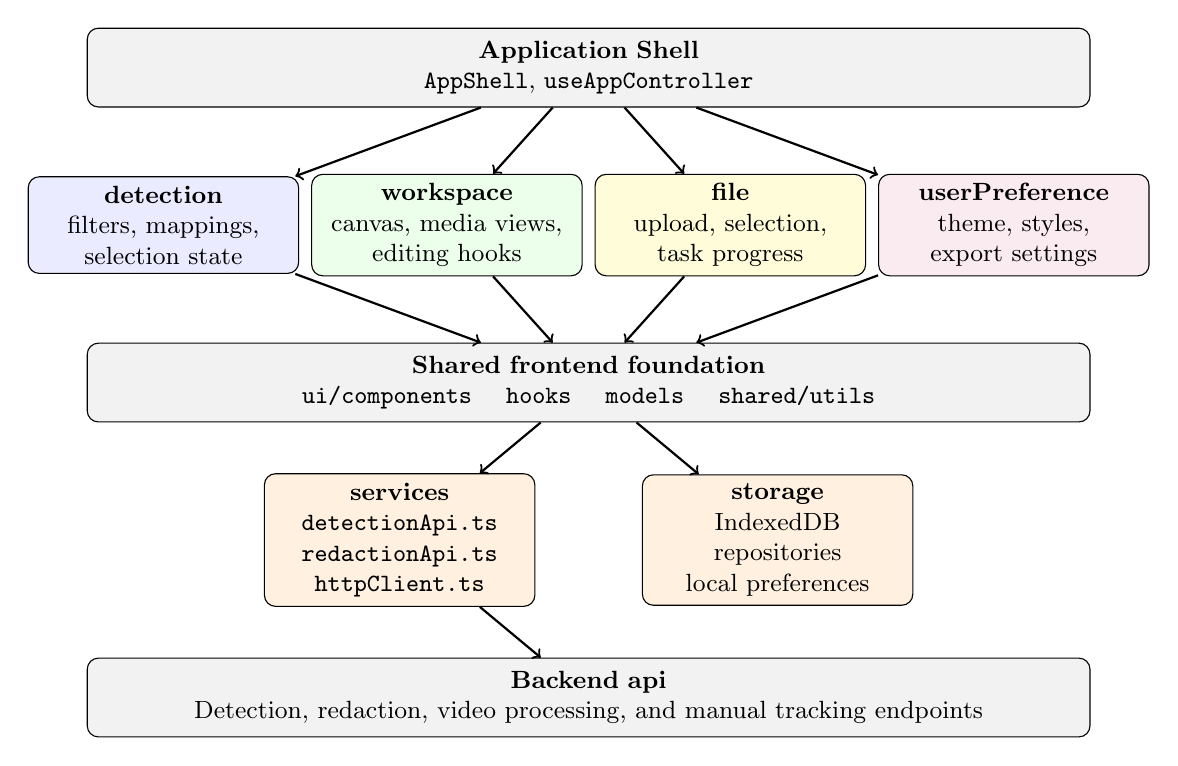
\begin{tikzpicture}[
    every node/.style={font=\small},
    box/.style={
        rectangle,
        rounded corners,
        draw=black,
        align=center,
        minimum height=1cm,
        text width=3.2cm
    },
    widebox/.style={
        rectangle,
        rounded corners,
        draw=black,
        align=center,
        minimum height=1cm,
        text width=12.5cm
    },
    arrow/.style={->, thick}
]

% Top level
\node[widebox, fill=gray!10] (app) at (0, 4)
{\textbf{Application Shell}\\
\texttt{AppShell}, \texttt{useAppController}};

% Feature modules
\node[box, fill=blue!8] (detection) at (-5.4, 2)
{\textbf{detection}\\
filters, mappings,\\
selection state};

\node[box, fill=green!8] (workspace) at (-1.8, 2)
{\textbf{workspace}\\
canvas, media views,\\
editing hooks};

\node[box, fill=yellow!15] (file) at (1.8, 2)
{\textbf{file}\\
upload, selection,\\
task progress};

\node[box, fill=purple!8] (prefs) at (5.4, 2)
{\textbf{userPreference}\\
theme, styles,\\
export settings};

% Shared layer
\node[widebox, fill=gray!10] (shared) at (0, 0)
{\textbf{Shared frontend foundation}\\
\texttt{ui/components} \quad \texttt{hooks} \quad \texttt{models} \quad \texttt{shared/utils}};

% Service and storage layer
\node[box, fill=orange!12] (services) at (-2.4, -2)
{\textbf{services}\\
\texttt{detectionApi.ts}\\
\texttt{redactionApi.ts}\\
\texttt{httpClient.ts}};

\node[box, fill=orange!12] (storage) at (2.4, -2)
{\textbf{storage}\\
IndexedDB repositories\\
local preferences};

% Backend
\node[widebox, fill=gray!10] (backend) at (0, -4)
{\textbf{Backend \acrshort{api}}\\
Detection, redaction, video processing, and manual tracking endpoints};

% Arrows
\draw[arrow] (app) -- (detection);
\draw[arrow] (app) -- (workspace);
\draw[arrow] (app) -- (file);
\draw[arrow] (app) -- (prefs);

\draw[arrow] (detection) -- (shared);
\draw[arrow] (workspace) -- (shared);
\draw[arrow] (file) -- (shared);
\draw[arrow] (prefs) -- (shared);

\draw[arrow] (shared) -- (services);
\draw[arrow] (shared) -- (storage);
\draw[arrow] (services) -- (backend);

\end{tikzpicture}

\caption{Feature-based frontend structure in \gls{SafeVision}. Domain-specific modules encapsulate their own components, hooks, state logic, and utilities, while shared UI elements, services, and storage repositories are reused across the application.}
\label{fig:frontend_structure}
\end{figure}

Shared functionality is implemented through a dedicated service layer located in the \texttt{services} directory. This includes modules such as \texttt{detectionApi.ts} and \texttt{redactionApi.ts}, which handle communication with the backend, as well as a centralized HTTP client, \texttt{httpClient.ts}, for managing requests. This ensures that networking logic is decoupled from UI components.

This structure realizes the separation of concerns described in Chapter~\ref{user_interface_and_usability} by keeping feature-specific logic separated from shared UI components, service communication, and storage mechanisms. As a result, the frontend can be maintained and extended without requiring changes across unrelated parts of the codebase.

\methodheading{State Management and Interaction Logic}

State management is implemented using custom React hooks and centralized stores. Hooks such as \texttt{useDetectionsStore}, \texttt{useHighlightsStore}, and \texttt{useImages} manage application state related to detection results, annotations, and uploaded files.

\begin{lstlisting}[language=javascript, caption={Per-file detection state managed through a custom hook}, label={lst:frontend_detection_store}]
type DetectionsStore = Record<string, Rect[]>;

export function useDetectionsStore(): DetectionsStoreApi {
  const [storeByFileKey, setStoreByFileKey] = useState<DetectionsStore>({});

  const get = useCallback(
    (fileKey: string | null) => {
      if (!fileKey) return [];
      return storeByFileKey[fileKey] ?? [];
    },
    [storeByFileKey],
  );

  const set = useCallback((fileKey: string, rects: Rect[]) => {
    setStoreByFileKey((prev) => ({ ...prev, [fileKey]: rects }));
  }, []);

  return { get, set, reset, dump, restore };
}
\end{lstlisting}

Listing~\ref{lst:frontend_detection_store} shows how detection results are stored per file key. This makes it possible to switch between uploaded media while keeping each file's detections separate. The state is updated immutably, which fits React's rendering model and makes the store compatible with undo and redo snapshots.

Since detection and highlight state are stored centrally, updates made in the workspace can be reflected immediately in related interface elements, such as filters, redaction controls, and preview components. For example, when a user modifies a \gls{bounding box} in the workspace, the updated region is available to the rest of the interface without requiring the user to manually reload or reprocess the image.

The system also includes undo and redo functionality through history-aware hooks, such as \texttt{useUndoRedoHistory}. This allows users to safely experiment with edits without losing previous states, which is particularly important in a workflow where users may need to manually correct automatically detected regions.

\methodheading{Workspace and Image Interaction}

A central part of the frontend is the workspace system, which provides an interactive canvas for image manipulation. Components such as \texttt{CanvasSurface}, \texttt{PageEditorSurface}, and \texttt{ImageWorkspace} enable rendering of images and overlaying of detection results, as illustrated earlier in Figure~\ref{fig:ui_final_examples}.

Detected regions are represented as \gls{bounding box}es, which can be selected, resized, moved, or deleted by the user. Interaction logic is handled through hooks such as \texttt{useHighlightBoxEditor} and \texttt{useImageBoxes}, which manage user input and coordinate transformations. Separating this logic into hooks prevents the canvas components from becoming responsible for both rendering and interaction state. This is important because editing operations all depend on consistent coordinate handling between the displayed image and the original media dimensions.

The system also supports zooming, panning, and precise editing through custom hooks, such as \texttt{useZoom} and \texttt{useCtrlDragPan}. These mechanisms improve usability when working with high-resolution images, where sensitive regions may be small or difficult to adjust at the default zoom level.

\methodheading{Detection Integration in the UI}

Detection results are integrated into the frontend through a dedicated service layer, primarily through \texttt{detectionApi.ts}. When a user uploads an image and starts detection, the image is sent to the backend, and the returned detections are stored in the detection state.

\begin{lstlisting}[language=javascript, caption={Frontend detection request through the service layer}, label={lst:frontend_detection_request}]
export async function detectObjects(
  file: Blob,
  mode: DetectMode = "all",
  scale: number = 1,
  adaptiveScaling?: boolean,
  multiOrientation?: boolean,
  usePreprocess: boolean = false,
  signal?: AbortSignal,
): Promise<DetectResponse> {
  if (file.size === 0) {
    throw new Error("No file uploaded");
  }

  if (scale <= 0 || scale > 4) {
    throw new Error("Scale must be between 0 and 4");
  }

  const formData = new FormData();
  formData.append("file", file, "image.png");

  return postForm<DetectResponse>("/detect", {
    formData,
    query: {
      types: mode,
      ...(adaptiveScaling ? { adaptive_scaling: true } : { scale: scale ?? 1 }),
      use_preprocess: usePreprocess,
      ...(multiOrientation ? { multi_orientation: true } : {}),
    },
    signal,
    parseAs: "json",
  });
}
\end{lstlisting}

Listing~\ref{lst:frontend_detection_request} shows how detection requests are isolated in the service layer. UI components do not construct HTTP requests directly; instead, they call a typed service function that validates the input, builds the multipart request payload, forwards detection options as query parameters, and returns a structured detection response.

The UI provides filtering and categorization tools, such as \texttt{DetectionFiltersSection} and \texttt{CategoryMultiSelect}, which allow users to control which types of detections are visible. This is important when multiple detection models are used, as it helps reduce visual clutter and makes it easier for users to review the categories of sensitive information that are relevant to the current task.

\methodheading{Redaction Workflow Implementation}

The redaction workflow is implemented through hooks such as \texttt{useImageRedaction} and \texttt{useWorkspaceRedaction}, which coordinate the transformation of selected regions. Users can apply redaction either based on detected regions, or manually by defining custom areas. Redaction parameters, such as blur or pixelation, are controlled through UI components in the sidebar.

Before redaction is sent to the backend, the frontend filters out disabled regions and converts the remaining \gls{bounding box}es from canvas coordinates back to original image coordinates. This conversion is necessary because the user edits boxes on a scaled canvas, while the backend must redact the original image data.

\begin{lstlisting}[language=javascript, caption={Preparing selected regions for image redaction}, label={lst:frontend_redaction_workflow}]
async function redact() {
  // Only user-approved regions are sent to the backend.
  const activeRects = visibleHighlights.filter(
    (r) => r.enabled !== false,
  );

  if (!activeRects.length || !imgEl || !canvasRef.current) {
    return;
  }

  const rectsOriginal = activeRects.map((r) => {
    // Convert from displayed canvas coordinates to original image coordinates.
    const transformed = canvasRectToOriginal({
      rect: r,
      canvas: canvasRef.current,
      imgEl,
    });

    return {
      ...r,
      ...transformed,
    };
  });

  await redactBackend(rectsOriginal);

  // Clear stale boxes after the image has been redacted.
  hl.reset();
  detectionsStore.reset(fileKey);
}
\end{lstlisting}

Listing~\ref{lst:frontend_redaction_workflow} shows how the frontend prepares redaction input after the user has reviewed the detected or manually added regions. Only enabled regions are included, and each region is transformed to match the original media dimensions before being sent to the backend. After a successful redaction, local highlights and detection results are cleared so that outdated \gls{bounding box}es are not shown on top of the newly redacted image.

The frontend ensures that redaction is applied only to the active regions selected or approved through the user workflow. This maintains user control and reduces the risk of unintended modifications. The final result can then be exported using utilities such as \texttt{canvasExporter.ts}, which prepares the redacted media for download. During this export process, image metadata is not preserved in the downloaded output, as discussed in Appendix~\ref{appsec:relevant_metadata_categories}. This occurs automatically as a result of the canvas-based export workflow, without requiring a separate metadata-stripping implementation.


\methodheading{File Handling and User Workflow}

File management is handled through the \texttt{file} module, which includes components such as \texttt{FilePanel} and \texttt{UploadDropzone}. Users can upload, organize, and switch between multiple images within the same session.

Custom hooks, such as \texttt{useFileUpload} and \texttt{useFileSelection}, manage file operations. This supports workflows where several files are processed in one session and provides visual feedback during longer running operations. By keeping file handling separate from detection and redaction logic, the frontend avoids coupling media management directly to processing functionality, making it easier to support future extensions such as additional file types, improved batch handling, or alternative upload mechanisms.

\methodheading{Client-Side Storage and Privacy Considerations}

To support privacy oriented data handling, the frontend uses client side storage mechanisms for preferences, workflow state, and annotation data. Annotation data such as image highlights is stored through IndexedDB repositories such as \texttt{highlightsIndexedDbRepository}, while user preferences are stored separately through the user preferences repository and browser local storage. This keeps these data types local to the browser rather than persistently storing them on the server. This supports the project’s data minimization strategy by limiting unnecessary server-side persistence and allows users to continue working with locally stored annotation data during a session without requiring all interaction state to be maintained by the backend.

\begin{lstlisting}[language=javascript, caption={Fail-safe IndexedDB persistence for highlights}, label={lst:indexeddb_highlights}]
async save(key: string, rects: Rect[]): Promise<void> {
  try {
    const dbp = getEditorDb();

    // In test mode or unsupported browsers, persistence is skipped safely.
    if (!dbp) return;

    const db = await dbp;
    await db.put(EDITOR_STORE_NAMES.imageHighlights, {
      fileKey: key,
      rects,
      updatedAt: Date.now(),
    });
  } catch (err) {
    // Storage failure should not block the editing workflow.
    console.warn("IndexedDB save failed:", err);
  }
}
\end{lstlisting}

Listing~\ref{lst:indexeddb_highlights} shows the fail-safe storage pattern used for client-side annotation persistence. If IndexedDB is unavailable or the write operation fails, the error is handled locally instead of interrupting the user workflow. This supports privacy-oriented data handling by keeping annotation data in the browser, while also allowing the application to degrade gracefully if local storage is unavailable.

\section{Backend Implementation}
\label{backend_implementation}

The backend of Safe Vision is implemented as a layered architecture consisting of an \acrshort{api} layer and a computation backend. While the overall architecture was introduced in Chapter~7, this section explains how the design is realized in the codebase. Controllers, services, and pipeline components are organized into separate modules, allowing request handling, application logic, and \acrshort{ml} processing to remain decoupled.

\methodheading{API Layer}

The \acrshort{api} layer handles requests from the frontend and acts as the main entry point to the backend. The application uses modular routing, with separate controllers for different processing tasks. Listing~\ref{lst:fastapi_routing} shows how middleware and routes are registered in the application.

\begin{lstlisting}[caption={FastAPI application structure and routing}, label={lst:fastapi_routing}]
app = FastAPI(
    title="Automatic Image Redaction API",
    lifespan=lifespan
)

app.add_middleware(
    CORSMiddleware,
    allow_origins=ALLOWED_ORIGINS,
    allow_credentials=True,
    allow_methods=["*"],
    allow_headers=["*"],
)

app.include_router(detect_router, prefix="/api", tags=["Detection"])
app.include_router(redact_router, prefix="/api", tags=["Redaction"])
app.include_router(video_detect_router, prefix="/api", tags=["Video"])
app.include_router(video_redact_router, prefix="/api", tags=["Video"])
\end{lstlisting}

\begin{lstlisting}[caption={Detection endpoint with parallel execution}, label={lst:detect_endpoint}]
@router.post("/detect")
async def detect(file: UploadFile, types: str = Query(default="face")):
    data = await file.read()
    img_array = np.frombuffer(data, np.uint8)
    img = cv2.imdecode(img_array, cv2.IMREAD_COLOR)

    tasks = []

    # Run selected detectors in worker threads to avoid blocking the API handler.
    if "face" in types:
        face_detector = get_face_detector()
        tasks.append(asyncio.to_thread(run_pipeline_on_image, img, face_detector))

    if "text" in types:
        text_engine = get_text_ocr()
        tasks.append(asyncio.to_thread(run_pipeline_on_image, img, text_engine))

    # Aggregate all selected detector outputs into one response.
    results = await asyncio.gather(*tasks)

    return {"live": results}
\end{lstlisting}

The endpoint implementation keeps request handling separate from the computational parts of the backend. Listing~\ref{lst:detect_endpoint} shows how selected detection tasks are dispatched concurrently and aggregated into a single response, reducing latency when multiple detection types are requested in the same call. For redaction requests, the same layer receives image data together with detection results, validates the input, and forwards it to the processing pipeline where the selected redaction configuration is applied.


\methodheading{Computation Backend}

The computation backend performs the core processing tasks of the system, including detection and redaction of sensitive information. Unlike the \acrshort{api} layer, it is responsible for image processing and \acrshort{ml} \gls{inference} rather than request handling. It is organized into two main components: the detection pipeline and the redaction processing module.

\subsubsection{Detection Pipeline}

The detection pipeline analyzes visual media and identifies sensitive entities such as faces, text, \gls{barcode}s, license plates, and objects. It supports multiple task-specific detectors within a shared processing flow.

Once uploaded, the image is processed through a sequence of steps that prepares the input, runs the selected models, and converts the outputs into a shared result format for later review and redaction. Processing begins with optional preprocessing, where the input image may be scaled or enhanced to improve detection performance, particularly for small or low-quality inputs. The preprocessed image is then passed to one or more task-specific detection models. When multiple detectors are selected, they can be executed concurrently to improve throughput. The outputs are subsequently aggregated and converted into a shared representation that standardizes bounding-box coordinates, confidence scores, and entity labels.

\begin{lstlisting}[caption={Detection pipeline processing and bounding box normalization}, label={lst:run_pipeline}]
def run_pipeline_on_image(img_proc, detector, *, total_scale=1.0):
    detections = detector.detect(img_proc) or []

    boxes_xyxy = []
    scores = []

    # Reverse the preprocessing scale so boxes match the original image.
    inv_scale = 1.0 / total_scale if total_scale != 0 else 1.0

    for d in detections:
        x1 = int(round(d.x1 * inv_scale))
        y1 = int(round(d.y1 * inv_scale))
        x2 = int(round(d.x2 * inv_scale))
        y2 = int(round(d.y2 * inv_scale))

        boxes_xyxy.append((x1, y1, x2, y2))
        scores.append(float(d.score))

    return boxes_xyxy, scores
\end{lstlisting}

Listing~\ref{lst:run_pipeline} shows how detections are converted into a normalized \gls{bounding box} representation. The detector output is first collected as coordinate pairs and confidence scores, before the coordinates are rescaled back to the original image dimensions using the inverse of the preprocessing scale. This ensures that detection results remain consistent with the original media, even when preprocessing has resized the image before \gls{inference}. The final output of the detection pipeline is a structured representation of the detected entities, which is returned to the \acrshort{api} layer for further processing or visualization in the frontend.

\subsubsection{Redaction Processing}

The redaction processing module anonymizes sensitive image regions based on the output of the detection pipeline. It applies \gls{masking} and transformation methods to the identified areas. It receives the original image together with the detected regions and prepares these inputs for redaction. Depending on the selected configuration, the system applies either \gls{bounding box} \gls{masking} or \gls{segmentation} based \gls{masking}. When \gls{segmentation} is enabled, \gls{mobilesam} is used to generate more precise masks for complex shapes, as illustrated in Figure~\ref{fig:segmentation_comparison} in Chapter~\ref{chap:results}.

Once the \gls{masking} regions have been defined, the selected \gls{anonymization} method is applied. Each supporting redaction method representing a different trade-off between privacy, visual quality, and computational cost. Listing~\ref{lst:redaction_method} shows how the available \gls{anonymization} methods are applied through a shared interface. After processing, the image may be resized and encoded into a standard output format before being returned to the \acrshort{api} layer. This supports compatibility with the frontend and efficient data transfer.

\begin{lstlisting}[caption={Application of redaction methods}, label={lst:redaction_method}]
def _apply_method(method, out, roi, mask, pixel_size, inpaint_radius, box_coords=None):
    if method == "blur":
        _apply_blur(roi, mask)
    elif method == "pixelate":
        _apply_pixelate(roi, mask, pixel_size)
    elif method == "blackbox":
        _apply_blackbox(roi, mask)
    elif method == "inpaint":
        _apply_inpaint_full_image(out, box_coords, mask)
    else:
        raise ValueError(method)
\end{lstlisting}






\section{\acrshort{ml} Model Development}

This section describes the development of the custom \acrshort{ml} models used in \gls{SafeVision} before their integration into the application backend. The main development effort concerned two image-based \gls{object detection} models for barcodes and license plates, while a separate \acrshort{ner} pipeline was developed to identify sensitive textual entities in \acrshort{ocr}-extracted text. Since these tasks required different training data, preprocessing steps, and evaluation methods, the code, scripts, and training workflows were kept in separate \acrshort{ml} development repositories rather than in the deployed \gls{SafeVision} application repository (Figure~\ref{fig:cv_repos}). This separation made it possible to isolate preprocessing, training, experimentation, and evaluation from the production application, while allowing the deployed system to remain focused on \gls{inference} and system integration.

\methodheading{Overview of Training Pipeline}

The training pipeline described in this section applies to both the \gls{barcode} and license plate detection models. For clarity, the \gls{barcode} and QR detection pipeline is used as the primary example, while the same overall process was also applied to the license plate model.

\begin{figure}[H]
\centering
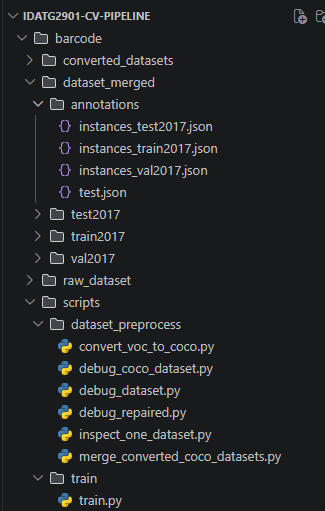
\includegraphics[width=\textwidth,height=0.40\textheight,keepaspectratio]{figures/images/chapter-8/cv_pipeline_structure.png}
\caption{Directory structure of the computer vision repository used for dataset preprocessing and model training.}
\label{fig:cv_pipeline_structure}
\end{figure}

The CV-repository, was structured to separate preprocessing, dataset management, and training into independent modules. This organization simplified experimentation and made it possible to reuse preprocessing steps across multiple training runs. The dataset followed a COCO-style structure with dedicated training, validation, and test splits together with corresponding annotation files. Preprocessing was handled by scripts in the \texttt{dataset\_preprocess} module, while model training was executed through the \texttt{train.py} entry point.

\methodheading{Dataset Preparation}

The dataset preparation process consisted of collecting multiple datasets from different sources, converting them into a unified annotation format, and merging them into a single dataset for training the \gls{barcode} detection model. Since few datasets were directly designed for \gls{barcode} and QR code detection, multiple sources were combined to construct a unified dataset (Table~\ref{tab:barcode_datasets}). Many existing datasets are intended for recognition rather than detection, which meant that several images either lacked suitable \gls{bounding box} annotations or required conversion to a detection format.

\begin{table}[H]
\centering
\begin{tabular}{|p{3.5cm}|p{3cm}|p{7.2cm}|}
\hline
\textbf{Dataset} & \textbf{Source} & \textbf{Description} \\ \hline

\textbf{archive\_1} & 
Kaggle \cite{barcode_qr_kaggle} & 
Collection of real-world \gls{barcode} and QR code images from diverse environments. \\ \hline

\textbf{\gls{barcode}\_bb, e8\_bb, multi\_bb} & 
Zenodo \cite{zenodo_barcode_datasets} & 
Benchmark datasets with \gls{bounding box} annotations for \gls{barcode} detection, including multiple instances per image. \\ \hline

\textbf{kaggle (InventBar, ParcelBar)} & 
Kaggle \cite{benchmark_barcode_kaggle} & 
Benchmark datasets containing \gls{barcode} images captured in industrial and logistics scenarios. \\ \hline

\textbf{syn10k\_plus\_huawei} & 
University of Szeged \cite{syn10k_dataset} & 
Synthetic \gls{barcode} dataset designed to increase data diversity and improve generalization. \\ \hline

\textbf{Total} & 
15731 & 
Combined into a unified dataset for training and evaluation. \\ \hline

\end{tabular}
\caption{Overview of datasets used for training the \gls{barcode} detection model.}
\label{tab:barcode_datasets}
\end{table}

In addition, most available datasets emphasize standard 1D \gls{barcode}s and QR codes, with more limited coverage of less common \gls{barcode} types. As a result, dataset preparation required substantial preprocessing, including annotation conversion, filtering, and merging of heterogeneous sources.

\begin{figure}[H]
\centering
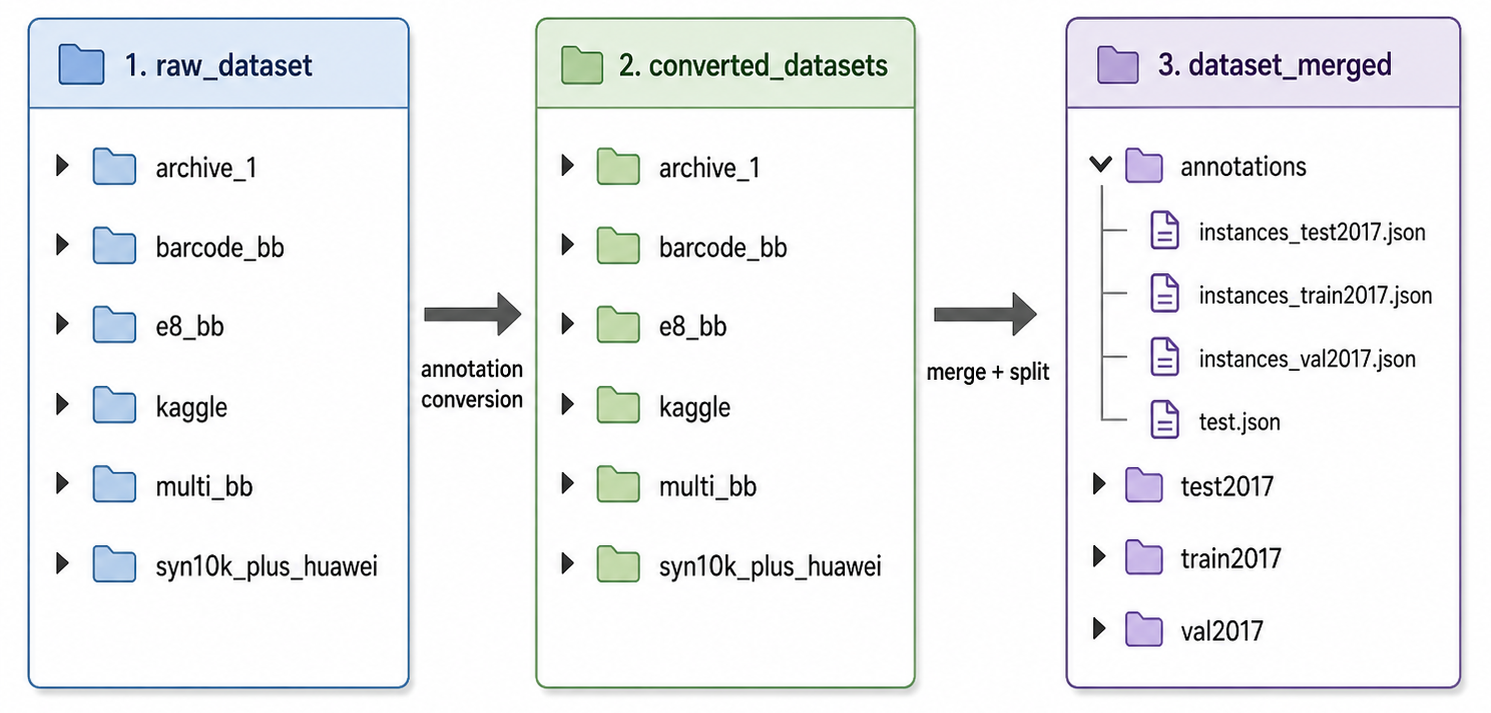
\includegraphics[width=\textwidth,height=0.25\textheight,keepaspectratio]{figures/images/chapter-8/dataset_preperation_pipeline.png}
\caption{Dataset preparation pipeline illustrating the transformation from raw datasets to a unified, merged, and split dataset used for training. Created by the au-
thors, with AI-assisted refinement}
\label{fig:dataset_preperation_pipeline}
\end{figure}

To ensure consistency across all data sources, each dataset was first converted into a unified annotation format. The datasets were then merged and divided into training, validation, and test subsets. As illustrated in Figure~\ref{fig:dataset_preperation_pipeline}, this process transformed raw datasets into a structured dataset suitable for training \gls{object detection} models. To maintain balanced source representation, the split was performed per dataset before the subsets were merged. This prevented larger datasets from dominating the final train, validation, and test distributions. Listing~\ref{lst:dataset_merge_split} shows the core splitting strategy used in the preprocessing script.

\begin{lstlisting}[caption={Per-dataset splitting strategy used during dataset merging}, label={lst:dataset_merge_split}]
def split_images_by_dataset(all_items):
    by_dataset = defaultdict(list)

    for item in all_items:
        by_dataset[item["dataset_name"]].append(item)

    train_items, val_items, test_items = [], [], []
    rng = random.Random(RANDOM_SEED)

    for dataset_name, items in by_dataset.items():
        # Shuffle each source separately so every dataset contributes to each split.
        rng.shuffle(items)

        n = len(items)
        n_train = int(n * TRAIN_RATIO)
        n_val = int(n * VAL_RATIO)

        train_items.extend(items[:n_train])
        val_items.extend(items[n_train:n_train + n_val])
        test_items.extend(items[n_train + n_val:])

    return train_items, val_items, test_items
\end{lstlisting}

This strategy ensured that each source dataset contributed samples to all splits while keeping the final dataset compatible with the \gls{yolox} training framework. The same preparation workflow was also applied to the license plate detection model. However, because the license plate dataset was built from fewer and more uniform sources, the \gls{barcode} dataset is used here as the main example. The complete license plate dataset split is reported in Appendix~\ref{app:license_plate_results}.

\methodheading{Data Augmentation}

Data augmentation was applied during training using the built-in online augmentation mechanisms provided by the \gls{yolox} framework. No separate offline augmentation pipeline was used. The augmentation strategy was intentionally kept relatively simple, since the training data already contained substantial variation across sources, including both synthetic and real-world images. This reduced the need for more aggressive augmentation methods.

\begin{lstlisting}[caption={\gls{yolox} augmentation configuration (excerpt)}, label={lst:yolox_aug}]
self.mosaic_prob = 0.0
self.mixup_prob = 0.0

self.hsv_prob = 0.5
self.flip_prob = 0.5

self.degrees = 5.0
self.translate = 0.05
self.shear = 1.0
\end{lstlisting}

\begin{figure}[H]
\centering
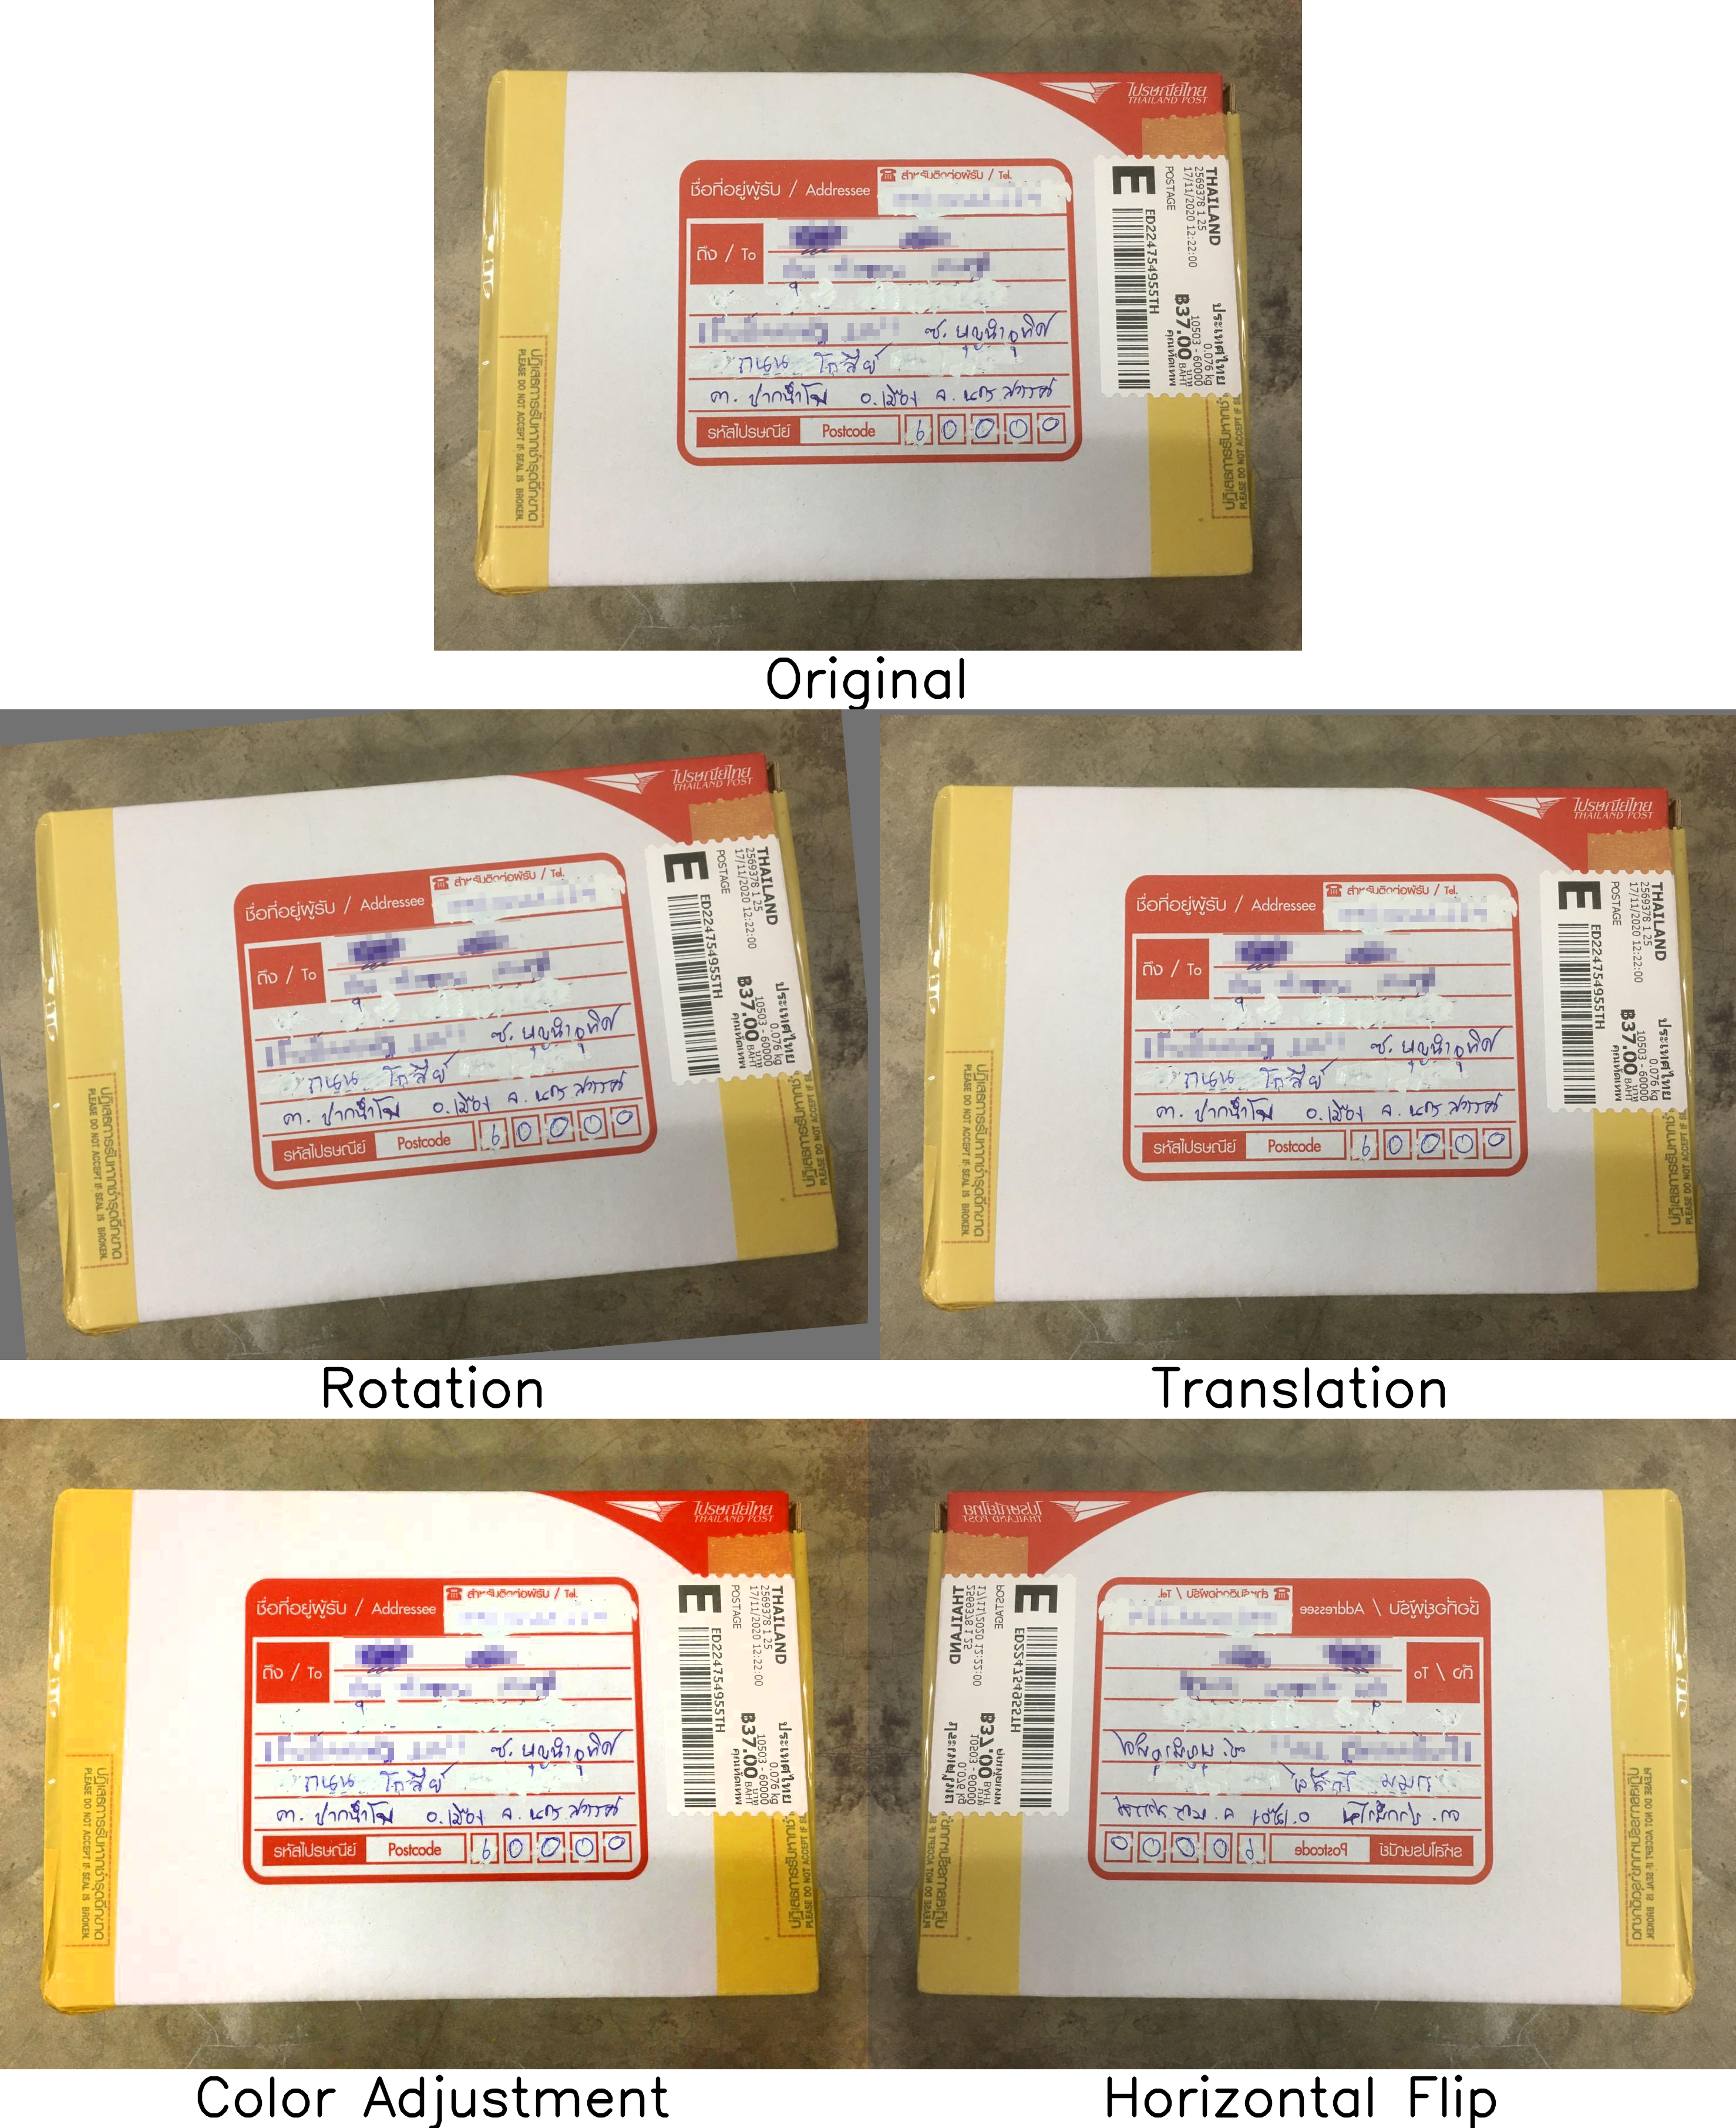
\includegraphics[width=0.7\textwidth]{figures/images/chapter-8/augmentations-example.png}
\caption{
Examples of geometric and photometric augmentations applied during training,
including rotation, translation, color adjustment, and horizontal flipping.
Image source ~\cite{inventbar_kaggle}.
}
\label{fig:data_augmentation_examples}
\end{figure}

The selected augmentations were intended to improve robustness to moderate variation in camera orientation, lighting conditions, and object placement while preserving the visual characteristics of \gls{barcode}s and license plates. The augmentation configuration was implemented directly in the \gls{yolox} experiment file. A simplified excerpt is shown in Listing~\ref{lst:yolox_aug}, while the full configuration is provided in Appendix~\ref{app:yolox_config}.

\methodheading{Model Training}

Model training was performed in \gls{yolox} using pretrained weights from the official \gls{yolox} repository \cite{yolox_github}. This reduced training time and provided a strong baseline for custom detector development. All models used the \gls{yolox-s} architecture. The shared training configuration included a base learning rate of \texttt{0.01 / 64}, 5 warmup epochs, a minimum learning rate ratio of \texttt{0.05}, SGD as optimizer, and 15 no-augmentation epochs.

Training was conducted on a system equipped with an NVIDIA RTX 4080 \gls{gpu} and 32 GB of RAM. As a result, some configuration choices, particularly input resolution and batch size, were selected not only based on validation performance but also to remain within the available memory budget and avoid instability or out-of-memory failures.

The main differences between model versions concerned input resolution, batch size, maximum number of epochs, and augmentation settings. These were adjusted through empirical experimentation in order to balance detection performance, training stability, and hardware constraints. A summary of the training configurations is provided in Appendix~\ref{app:custom_model_evaluation}, while the complete configuration details are included in Appendix~\ref{app:yolox_config}.

\subsubsection{Named Entity Recognition Model Development}

In addition to the image-based object detectors, the project also included the development of a custom named entity recognition (NER) pipeline for detecting sensitive textual information extracted through \acrshort{ocr}. While the \gls{barcode} and license plate models addressed a visual detection problem, the NER component addressed a text understanding problem by identifying sensitive entities directly in recognized text.

The purpose of the NER pipeline was to classify \acrshort{ocr} extracted text into privacy-relevant categories as shown in List~\ref{lst:ner_label_maps}. This made it possible to extend text handling beyond pure \acrshort{ocr} extraction by adding semantic interpretation of the recognized content.

\begin{lstlisting}[caption={BIO label construction for NER training}, label={lst:ner_label_maps}]
ENTITY_LABELS = [
    "PERSON_NAME",
    "PHONE",
    "EMAIL",
    "DATE",
    "ADDRESS",
    "LOCATION",
    "LICENSE_PLATE",
    "POSTAL_CODE",
    "URL",
    "ORGANIZATION",
    "ID_NUMBER",
]
\end{lstlisting}

\methodheading{Dataset Construction}

Since no directly suitable domain-specific dataset was available for all target categories, the NER training data was constructed by combining synthetically generated samples with converted external NER datasets. The synthetic dataset generation pipeline was implemented in \texttt{dataset\_gen.py}, where entity values were sampled from predefined generators and inserted into template-based text examples.

To improve robustness, the generated data included both Norwegian and English text, \acrshort{ocr} like distortions, formatting variation, random casing, typographical noise, and hard negative examples. In addition to short field-based examples, the generator also produced chat-style, form-style, report-style, and document-style samples to better reflect the variability of \acrshort{ocr} derived text in practice.

To strengthen recognition of general linguistic entity categories, two external NER datasets were incorporated into the workflow. The Norwegian NorNE corpus and an English NER dataset were converted into the project’s internal JSONL format and mapped to the \gls{SafeVision} entity schema. These external datasets primarily strengthened recognition of person names, organizations, and locations in natural running text, while the synthetic dataset remained responsible for \acrshort{ocr} specific and privacy specific entity categories such as phone numbers, email addresses, URLs, postal codes, license plates, and identification numbers.

After conversion, the synthetic and external datasets were merged and subsequently divided into training, validation, and test subsets. Detailed dataset composition and split sizes are provided in Appendix~\ref{app:ner_evaluation}.

\methodheading{NER Model Training}

The NER model was trained using XLM-RoBERTa as the encoder backbone through the Hugging Face Transformers framework. The implementation in \texttt{train\_ner.py} used a token classification setup, where each token was assigned a BIO-formatted label corresponding to the underlying entity category.

During preprocessing, character-level entity spans were aligned to tokenizer offsets. Tokens outside annotated spans were assigned the \texttt{O} label, while tokens inside an entity span were assigned \texttt{B-} and \texttt{I-} prefixes depending on whether the token started or continued the entity.
Listning~\ref{ner_align_labels}
\begin{lstlisting}[caption={Span-to-token alignment for BIO labeling}, label={lst:ner_align_labels}]
def align_labels(example, tokenizer, max_length):
    encoding = tokenizer(
        example["text"],
        truncation=True,
        max_length=max_length,
        return_offsets_mapping=True,
    )

    offsets = encoding["offset_mapping"]
    labels = []

    for token_start, token_end in offsets:
        if token_start == token_end:
            labels.append(-100)
        else:
            labels.append(label2id["O"])

    for ent in example["entities"]:
        start, end, label = ent["start"], ent["end"], ent["label"]

        first = True
        for i, (token_start, token_end) in enumerate(offsets):
            if token_start == token_end:
                continue

            if token_start < end and token_end > start:
                prefix = "B" if first else "I"
                labels[i] = label2id[f"{prefix}-{label}"]
                first = False

    encoding["labels"] = labels
    encoding.pop("offset_mapping")
    return encoding
\end{lstlisting}

Training was performed using the Hugging Face \texttt{Trainer} \acrshort{api} with a token classification model initialized from \texttt{FacebookAI/xlm-roberta-base}. The detailed training configuration and evaluation results are provided in Appendix~\ref{app:ner_evaluation}.

\methodheading{\Gls{inference} and Post-Processing}

After training, prediction and evaluation were performed through \texttt{predict\_ner.py}. The token-level predictions produced by the model were merged back into entity spans by grouping adjacent subword predictions and converting them to character offsets in the original text.

\begin{lstlisting}[caption={Merging token predictions into entity spans}, label={lst:ner_merge_spans}]
def merge_subword_spans(labels, offsets, probs, text, threshold=0.0):
    entities = []
    current = None

    for label, (start, end), score in zip(labels, offsets, probs):
        if start == end:
            continue

        if label == "O" or score < threshold:
            if current is not None:
                entities.append(current)
                current = None
            continue

        if "-" in label:
            prefix, entity_type = label.split("-", 1)
        else:
            prefix, entity_type = "B", label

        if prefix == "B":
            if current is not None:
                entities.append(current)
            current = {
                "start": start,
                "end": end,
                "label": entity_type,
                "scores": [score],
            }

        elif prefix == "I":
            if current is not None and current["label"] == entity_type:
                current["end"] = max(current["end"], end)
                current["scores"].append(score)
\end{lstlisting}

\acrshort{ocr} derived text often contains noise, inconsistent punctuation, and formatting wrappers, the raw spans were further post-processed before final evaluation. This included trimming punctuation, removing common textual prefixes such as field labels, stripping suffix wrappers, and applying lightweight heuristics for labels such as listed in Listning~\ref{lst:ner_align_labels}.

In the final system, the NER model complemented the \acrshort{ocr} subsystem by adding a text-level interpretation layer for privacy-sensitive content, but it was not used as a standalone text classification component. Instead, \acrshort{ocr} extracted text was processed through a hybrid text-analysis pipeline, implemented in
\texttt{pii\_detector.py} (Appendix~\ref{app:pii_detector}), where NER predictions were combined with contextual rules and post-processing heuristics. This was done because standalone NER predictions were less reliable on practical document inputs than the constructed evaluation results initially
suggested.

\section{AI/\acrshort{ml} Integration}
\label{ai_ml_integration}
This section describes how \acrshort{ml} models are integrated into the system to support detection of sensitive information. It outlines the structure of the detection engine and the strategy used to load and execute the individual models.

\methodheading{Detection Engine Architecture}

The detection engine combines several task-specific \acrshort{ml} models within a common framework. Each model is responsible for detecting a distinct category of sensitive information. An overview of the detection models and their capabilities is shown in Table~\ref{tab:detection_models}.

\begin{table}[H]
\centering
\small
\begin{tabularx}{\textwidth}{|p{2.7cm}|p{4.4cm}|X|}
\hline
\textbf{Engine} & \textbf{Technology} & \textbf{Capabilities} \\ \hline

\textbf{RetinaFace} & 
CNN-based face detector & 
Face detection with high accuracy and robustness to scale and pose. \\ \hline

\textbf{PaddleOCR} & 
\acrshort{ocr} framework (detection + recognition) & 
Text detection and recognition in natural scenes. \\ \hline

\textbf{XLM-RoBERTa NER} & 
Transformer-based token classification model & 
Identification of sensitive entities in \acrshort{ocr} extracted text. \\ \hline

\textbf{YOLOX} & 
Real-time \gls{object detection} (YOLO-based) & 
\gls{barcode}, license plate, and general \gls{object detection}. \\ \hline

\end{tabularx}
\caption{Overview of AI/\acrshort{ml} models used in the system.}
\label{tab:detection_models}
\end{table}

Although the models serve different tasks, they are integrated into a shared processing workflow. The image-based models operate on comparable visual inputs, while the NER model processes text extracted through \acrshort{ocr}. Their outputs are subsequently normalized into a shared representation that supports downstream filtering, review, and redaction. This simplifies integration and makes it easier to extend the system with additional detectors or text-analysis components. The detection engine is integrated with the processing pipeline described in Section~\ref{Preprocessing_subsection} and Section~\ref{subsec:post_processing}, where preprocessing, \gls{inference}, and post-processing are handled in sequence.

\methodheading{Model Integration and Execution}

The models follow a common integration pattern in order to keep the system simple and maintainable. Each detector is implemented in its own module, while model instances are loaded as shared resources to avoid repeated initialization. Therefore lazy loading is used to defer model initialization until a detector is first requested. This is implemented through helper functions such as \texttt{get\_face\_detector()} in \texttt{backend/controllers/detect\_controller.py}, which create the model instance on first use and return the same instance for subsequent requests.

\begin{lstlisting}[caption={Lazy loading of detection model}, label={lst:lazy_loading}]
def get_face_detector():
    global detector
    if detector is None:
        detector = load_model()
    return detector
\end{lstlisting}

Listing~\ref{lst:lazy_loading} shows how model initialization is deferred until first use and how the same instance is reused across requests. This structure improves code organization and makes it possible to add new detectors without requiring major changes elsewhere in the backend.

\section{Image Processing and Redaction Pipeline}
\label{image_processing_and_redaction_pipeline}

This section describes the processing steps applied to image data before and after model \gls{inference}. While the detection pipeline (Section~8.3.2) focuses on identifying sensitive entities, this component is responsible for preparing input data, transforming detection results, and applying \gls{anonymization} techniques. The implementation is primarily located in the pipeline modules under \texttt{pipeline/common}.


\methodheading{Preprocessing}
\label{Preprocessing_subsection}

The preprocessing stage prepares input images before they are passed to the detection models. This includes optional scaling and enhancement operations, which can improve detection accuracy, particularly for small or low-resolution objects. Scaling is used to balance performance and accuracy, where downscaling can reduce computation time and upscaling can improve detection of small features. Preprocessing operations are shared across multiple detection modules and ensure that all models operate on a consistent input representation.

In addition to manual scaling, the system supports adaptive scaling based on the requirements of individual detection models. When enabled, the image is automatically resized such that its resolution better matches the expected input size of the selected model. This is implemented through a model-aware preprocessing step, where the scaling factor is computed dynamically based on the model’s preferred input resolution. Listing~\ref{lst:adaptive_preprocessing} shows how adaptive scaling is integrated with the standard preprocessing pipeline. The system adjusts image resolution based on the selected model, while still reusing the same preprocessing logic.

\begin{lstlisting}[caption={Model-aware preprocessing with adaptive scaling}, label={lst:adaptive_preprocessing}]
def preprocess_for_model(
    img_bgr,
    h0,
    w0,
    model_name,
    adaptive_scaling,
    base_scale,
    use_preprocess,
):
    if adaptive_scaling:
        model_input = MODEL_INPUT_SIZES.get(model_name, 640)
        scale = model_input / max(h0, w0)
        scale = max(0.5, min(scale, 2.0))
    else:
        scale = base_scale

    img_proc, total_scale, used_preprocess = preprocess_image(
        img_bgr,
        scale=scale,
        use_preprocess=use_preprocess,
    )

    return img_proc, total_scale, used_preprocess
\end{lstlisting}

Adaptive scaling can improve detection accuracy, particularly for models that are sensitive to input resolution. However, it introduces additional computational cost due to image resizing. For this reason, it is implemented as an optional feature that can be enabled or disabled by the user. By default, adaptive scaling is enabled to prioritize detection accuracy, while still allowing performance-oriented configurations.

\methodheading{Bounding Box Processing}
\label{subsec:post_processing}

After detection, \gls{bounding box} processing is performed as a post-processing step to normalize outputs from different models into a unified format. This involves validating coordinates, clamping values to image boundaries, and ensuring that all \gls{bounding box}es are well-formed. The process also includes geometric transformations such as scaling and coordinate adjustment, which are necessary when preprocessing steps modify the image resolution. Additionally, \gls{bounding box}es may be expanded to include contextual regions, which is useful for \gls{segmentation} based \gls{masking}. These operations are implemented through utility functions that ensure robustness against invalid or out-of-bounds detections.

\methodheading{\Gls{segmentation} and Mask Generation}

To enable more precise redaction, the system supports \gls{segmentation} based \gls{masking} using \gls{mobilesam}. When \gls{segmentation} is requested, the system extracts a region of interest around the detected \gls{bounding box} and uses it as input to the \gls{segmentation} model. The resulting binary mask represents the object more accurately than a rectangular \gls{bounding box}, allowing for higher quality \gls{anonymization}.

The implementation includes several safeguards to ensure stability. If the \gls{segmentation} model is unavailable or fails to produce a valid mask, the system automatically falls back to \gls{bounding box} \gls{masking}. The generated masks are further refined using morphological operations, such as opening, closing, and smoothing, to remove noise and improve visual quality. Listing~\ref{lst:mask_refinement} illustrates how mask refinement is implemented in \texttt{anonymize.py}.

\begin{lstlisting}[caption={Mask refinement using morphological operations}, label={lst:mask_refinement}]
kernel = np.ones((5, 5), np.uint8)
mask = cv2.morphologyEx(mask, cv2.MORPH_OPEN, kernel)
mask = cv2.morphologyEx(mask, cv2.MORPH_CLOSE, kernel)
mask = cv2.GaussianBlur(mask, (9, 9), 0)
\end{lstlisting}

\methodheading{Redaction Methods}

This stage of the pipeline applies \gls{anonymization} to the detected regions. The functionality is implemented in \texttt{anonymize.py}, which provides a common interface for different redaction methods. The system supports blurring, pixelation, black-box \gls{masking}, and \gls{inpainting}. These methods are applied to selected regions using masks to blend the result with the original image.

\begin{lstlisting}[caption={Applying redaction to detected regions}, label={lst:anonymize_call}]
def anonymize(img, boxes, method="blur", mask_mode="segmentation"):
    out = img.copy()

    for box in boxes:
        roi_data = _get_roi_and_mask(img, out, box, pad_ratio=0.05, mask_mode=mask_mode)
        if roi_data is None:
            continue

        box_coords, roi, mask = roi_data

        _apply_method(method, out, roi, mask, pixel_size=40, inpaint_radius=7, box_coords=box_coords)

    return out
\end{lstlisting}

Listing~\ref{lst:anonymize_call} shows how redaction methods are applied to detected regions. For each \gls{bounding box}, a region of interest and corresponding mask are extracted, after which the selected \gls{anonymization} method is applied. This design enables flexible and consistent processing across different \gls{masking} strategies.

\begin{table}[H]
\centering
\begin{tabular}{lcc}
\hline
\textbf{Method} & \textbf{Visual Effect} & \textbf{Use Case} \\
\hline
Blur & Smooth distortion & Faces / privacy-friendly \gls{masking} \\
Pixelate & Block-based \gls{masking} & Strong \gls{anonymization} \\
Blackbox & Full occlusion & Maximum privacy \\
Inpaint & Background reconstruction & Aesthetic output \\
\hline
\end{tabular}
\caption{Comparison of redaction methods.}
\label{tab:redaction_methods}
\end{table}

Table~\ref{tab:redaction_methods} summarizes the available methods and their typical use cases. Blurring and pixelation reduce detail while keeping the general structure of the image. Black-box \gls{masking}, on the other hand, completely hides the selected region. \Gls{inpainting} works differently by filling the region using surrounding pixel information.

The system supports both \gls{bounding box} and \gls{segmentation} masks, and allows different methods to be applied to different regions. This makes it possible to balance privacy and visual quality depending on the  case.



\section{Video Implementation}
\label{sec:video_imp}

This section describes how video processing was implemented in \gls{SafeVision}. It explains how videos are decoded, how \gls{bounding box}es are propagated between detection frames and how the manual video tracking is handled.

\methodheading{Video Detection Integration}

Video detection is handled through the \texttt{POST /api/video/detect} endpoint and is implemented through \texttt{video\_detect\_controller.py} together with additional functionality. Uploaded videos are first stored in a temporary working directory before OpenCV is used to open the file and read video metadata. Using this method, \gls{SafeVision} can decode the video frame by frame by reading the frame rate and dimensions. Detection is not performed on every frame. The video iteration is handled by \texttt{iter\_video\_live} and the wrapper \texttt{extract\_video\_live}, while \texttt{detect\_live\_on\_frame} applies detection to the selected frames.

The frame-level detection function uses the same detection infrastructure as the image pipeline, including all preprocessing and models. This means that video does not use its own separate detection system, but instead applies the image-based detection already implemented in \gls{SafeVision} repeatedly to decoded frames. The result is returned as a manifest of all frames with a frame index, frame timestamp and a list of detections. This manifest is later used to create \gls{bounding box}es for review and redaction in a similar way as for images.

\methodheading{Prediction and Bounding Box Propagation}

As previously stated, the video pipeline does not run full image detection on every frame by default. Since \gls{SafeVision} reuses the same detectors for images and video, full detection on every frame can be computationally expensive. Therefore, an option is implemented for the user to decide the program's detection frequency. This is handled through the \texttt{detect\_every} parameter, which specifies detection on every Nth frame. A lower value runs detection more frequently, allowing the user to balance processing time against video detection accuracy.

Between detection frames, \gls{bounding box}es are propagated using \texttt{kalman\_multi\_tracker.py}. This implementation follows the video tracking approach introduced in Section~\ref{sec:video_tracking_foundation}, where Kalman-based prediction, entity-specific matching, interpolation, and backfilling are used to maintain temporally consistent \gls{bounding box}es between sparse detection frames. For each frame, the \gls{kalman filter} predicts the next position of active \gls{bounding box}es based on their previous location and movement. This allows detected regions to remain present in frames where the detector is not executed, reducing the risk that sensitive content disappears between detection intervals.

When a new detection frame is reached, the backend runs \texttt{detect\_live\_on\_frame(...)} and matches the new detections with existing predicted boxes. This matching is performed separately for each entity type. If a new detection matches an existing prediction, the \gls{kalman filter} corrects the predicted position using the detected box. If a detection does not match any existing prediction, a new prediction state is created, indicating that a new sensitive object may have appeared in the video. Prediction states that remain unmatched for too long are eventually stopped, since this indicates that the object is no longer visible. This flow is illustrated in Figure~\ref{fig:video_tracking_flow}.

\begin{figure}[H]
\centering
\begin{tikzpicture}[
    every node/.style={font=\small},
    box/.style={
        rectangle,
        rounded corners,
        draw=black,
        minimum width=4.0cm,
        minimum height=0.75cm,
        align=center
    },
    widebox/.style={
        rectangle,
        rounded corners,
        draw=black,
        minimum width=5.4cm,
        minimum height=0.75cm,
        align=center
    },
    decision/.style={
        diamond,
        draw=black,
        aspect=2,
        align=center,
        inner sep=1pt,
        minimum width=2.8cm,
        minimum height=1.1cm
    },
    arrow/.style={->, thick}
]

% Nodes with fixed coordinates
\node[box]      (read)     at (0, 0)      {Read frame};
\node[box]      (predict)  at (0, -1.3)   {Predict active boxes};
\node[decision] (detectq)  at (0, -2.8)   {Is this a\\ detection frame?};

\node[box]      (detect)   at (-3.4, -4.2) {Run frame-level detectors};
\node[box]      (match)    at (-3.4, -5.4) {Match and update boxes};

\node[box]      (usepred)  at (3.4, -4.2)  {Use predicted boxes};

\node[widebox]  (manifest) at (0, -6.8)    {Write active boxes to frame manifest};

% Arrows
\draw[arrow] (read) -- (predict);
\draw[arrow] (predict) -- (detectq);

\draw[arrow] (detectq) -- node[above left] {Yes} (detect);
\draw[arrow] (detect) -- (match);

\draw[arrow] (detectq) -- node[above right] {No} (usepred);

\draw[arrow] (match.south) |- (manifest.west);
\draw[arrow] (usepred.south) |- (manifest.east);

\end{tikzpicture}
\caption{Simplified flow of video detection and prediction. For each frame, the \gls{kalman filter} first predicts active regions. If the frame is selected for detection, frame-level detectors are executed and matched with existing predictions. Otherwise, the predicted boxes are used directly before the frame data is written to the manifest.}
\label{fig:video_tracking_flow}
\end{figure}

\methodheading{Manual Tracking}

Manual tracking is handled separately from the automatic Kalman-based prediction. For images, manual boxes are drawn and can be redacted directly, but in video a manually drawn box would either only affect the single frame where it was drawn or remain as a stationary box over a span of frames. Therefore, to make manual redaction usable for video, \gls{SafeVision} includes a dedicated manual tracking endpoint, \texttt{POST /api/video/track-manual}. This endpoint receives the video and the existing manifest, regardless of whether it already contains Kalman-predicted boxes, and adds the manually tracked region across the relevant frames. The implementation is mainly located in \texttt{video\_track\_manual\_controller.py} and \texttt{manual\_single\_tracker.py}.

Manual tracking is handled by \texttt{track\_manual\_box\_in\_manifest}, which initializes tracking from the selected frame and the region selected by the user. Unlike the automatic Kalman-based prediction, this manual tracking path uses an OpenCV object tracker to follow the user-defined region through the video. The implementation primarily uses TrackerViT, while Channel and Spatial Reliability Tracking (CSRT) is included as a fallback tracker. This connects the implementation to the tracking methods introduced in Section~\ref{sec:video_tracking_foundation}. The selected region is tracked both forward and backward from the chosen frame, and manual tracks are assigned negative track IDs so that they do not collide with automatically generated track IDs.

\begin{figure}[H]
\centering

\begin{subfigure}{0.48\textwidth}
    \centering
    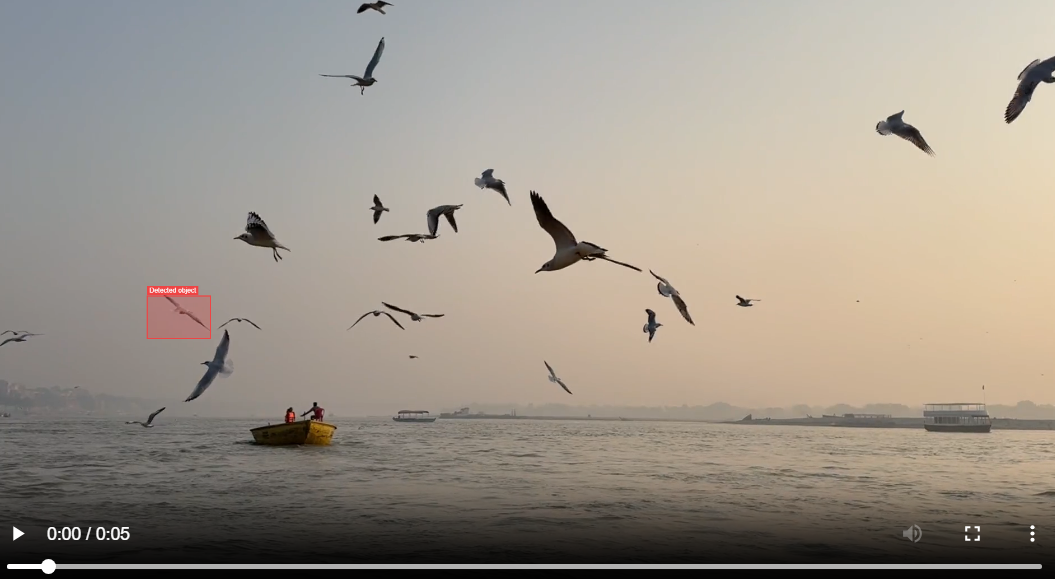
\includegraphics[width=\textwidth]{figures/images/chapter-8/bird1.png}
    \caption{Manual \gls{bounding box} initialized on a bird in the selected frame.}
\end{subfigure}
\hfill
\begin{subfigure}{0.48\textwidth}
    \centering
    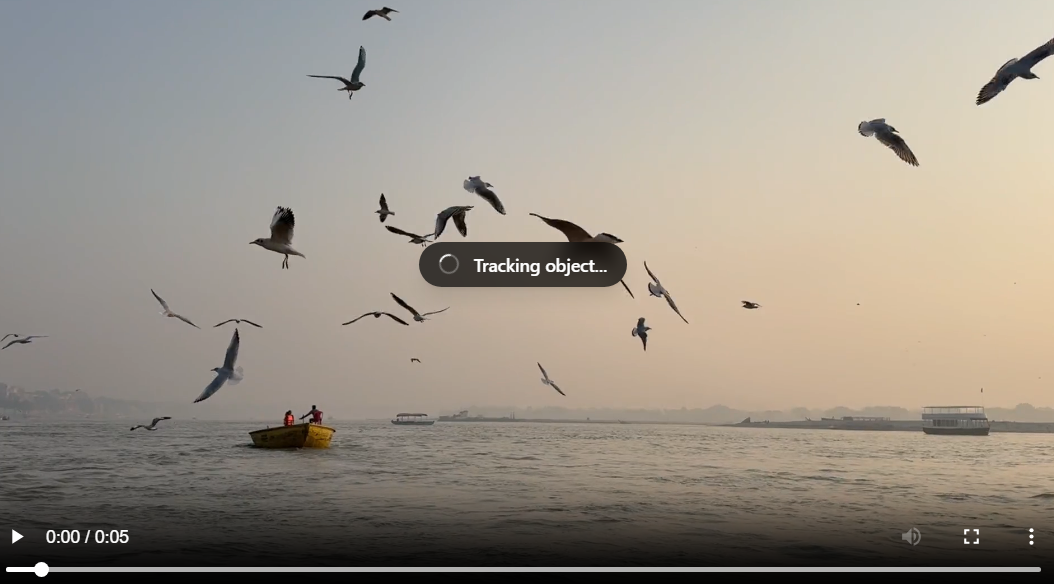
\includegraphics[width=\textwidth]{figures/images/chapter-8/bird2.png}
    \caption{Tracker propagated to other frames in the video.}
\end{subfigure}

\vspace{0.4cm}

\begin{subfigure}{0.48\textwidth}
    \centering
    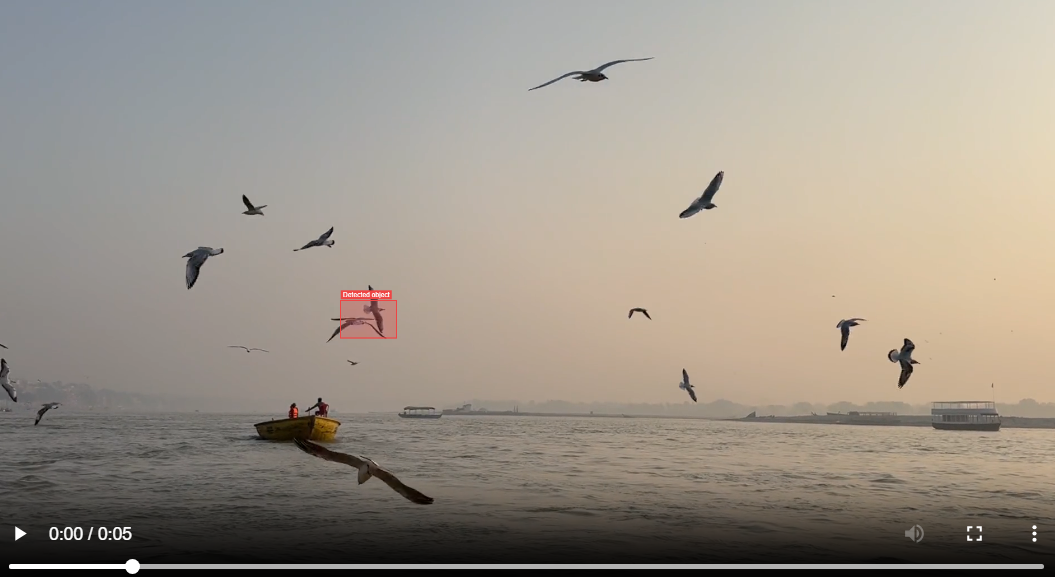
\includegraphics[width=\textwidth]{figures/images/chapter-8/bird3.png}
    \caption{Bird flies through an area with low tracking certainty.}
\end{subfigure}
\hfill
\begin{subfigure}{0.48\textwidth}
    \centering
    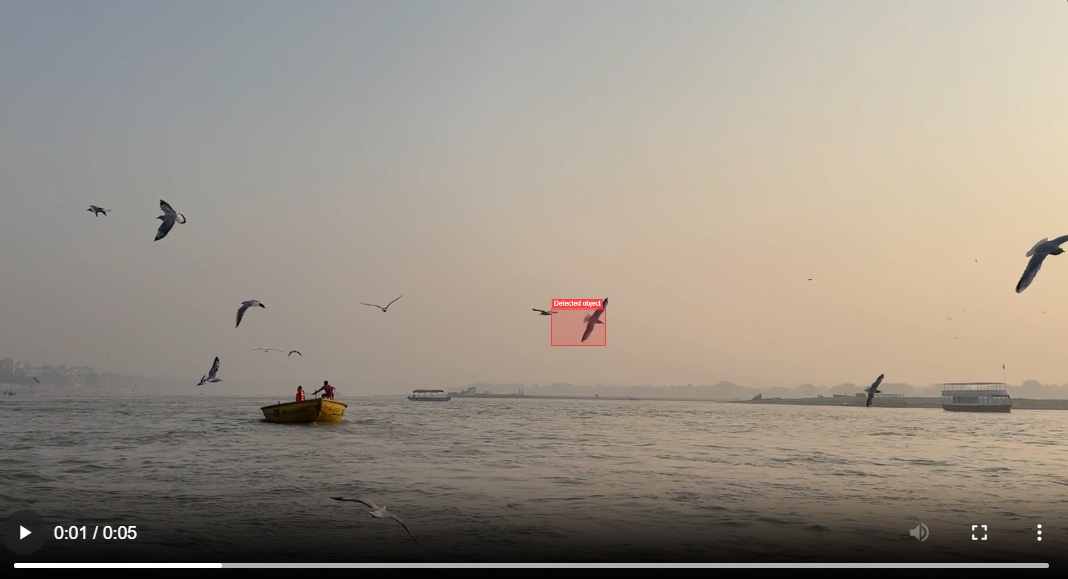
\includegraphics[width=\textwidth]{figures/images/chapter-8/bird4.png}
    \caption{Successfully tracked the bird through the flock.}
\end{subfigure}

\caption{Example of manual video tracking in \gls{SafeVision}. A manually drawn \gls{bounding box} is initialized on one frame and propagated through later frames. Source video by~\cite{pexels_shubh_agrawal_video}.}
\label{fig:manual_video_tracking_sequence}
\end{figure}


The manual tracking implementation includes safeguards to reduce unstable tracking results from either TrackerViT or the \acrshort{csrt} fallback. Functions such as \texttt{\_is\_suspicious} and \texttt{\_replay\_safety\_candidate} are used when the tracker output appears unreliable. These checks handle sudden changes in size or aspect ratio, large jumps in position, weak overlap with the last trusted box, or abnormal growth of the tracked object near the frame border. When tracking gives low certainty, the system can temporarily keep the last trusted box, add only the new predicted area of the tracked object as a union, and later replay tracking from a safer region. This makes the manual tracking more reliable than applying raw tracker output directly.

\methodheading{Video Redaction Pipeline}

Video redaction is handled through the \texttt{POST /api/video/redact} endpoint and is controlled through \texttt{video\_redact\_controller.py}. When redaction is run, it receives the original video together with the frame-wise manifest as a blueprint for what to redact. The backend reads the video frame by frame and matches each frame with the corresponding detections listed in the manifest using the function \texttt{redact\_frame\_with\_live}.

The function \texttt{redact\_frame\_with\_live} reuses the existing redaction logic through \texttt{anonymize}, allowing the video pipeline to use the same methods and settings as for images. This means that a video can use blackbox, blur, pixelation, \gls{inpainting} and \gls{segmentation} for the relevant box categories. After processing all frames, OpenCV is used to write a temporary video output, and \texttt{remux\_to\_h264\_aac} in \texttt{ffmpeg\_utils.py} finalizes the complete redacted video before temporary files are cleaned up.


\section{Deployment}

This section describes how the deployment architecture and infrastructure presented in Chapter~\ref{chap:technologies_and_methodologies} (Figure~\ref{fig:deployment_architecture}) are implemented in practice. The deployment setup ensures reproducibility, scalability, and efficient handling of both frontend and backend components.

\methodheading{Continuous Integration and Deployment}

The system uses GitHub Actions to implement both continuous integration (CI) and continuous deployment (CD) as part of the development workflow.

\begin{figure}[H]
    \centering
    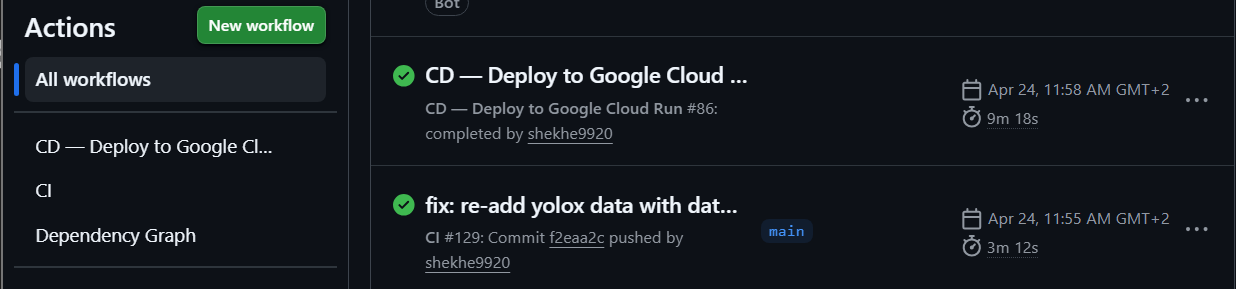
\includegraphics[width=0.85\textwidth]{figures/images/chapter-8/github-actions-workflow.png}
    \caption{Example of successful CI and CD workflow executions in GitHub Actions. The workflows were used to validate frontend and backend changes before deploying updated application artifacts.}
    \label{fig:github_actions_workflow}
\end{figure}

\paragraph{Continuous Integration (CI)}

The CI pipeline is triggered on every push or pull request to the main branch and is responsible for validating both frontend and backend components. For the frontend, the pipeline installs dependencies using npm, performs linting and type checking, runs tests, and builds the application to ensure that the code compiles correctly. For the backend, the pipeline installs Python dependencies, performs static analysis using Ruff, and executes unit tests using pytest. To enable testing without requiring \acrshort{ml} model weights, a configuration flag (\texttt{ALLOW\_FAKE\_DETECTORS}) is used to bypass model loading during CI execution. An excerpt of the CI pipeline is shown in Listing~\ref{lst:ci_pipeline}.

\begin{lstlisting}[caption={Excerpt from CI pipeline using GitHub Actions}, label={lst:ci_pipeline}]
jobs:
  frontend:
    runs-on: ubuntu-latest
    steps:
      - uses: actions/checkout@v4
      - uses: actions/setup-node@v4
      - run: npm ci
      - run: npm run lint --if-present
      - run: npm test --if-present
      - run: npm run build

  backend:
    runs-on: ubuntu-latest
    env:
      ALLOW_FAKE_DETECTORS: "true"
    steps:
      - uses: actions/checkout@v4
      - uses: actions/setup-python@v5
      - run: pip install -r requirements.txt
      - run: ruff check .
      - run: pytest -q
\end{lstlisting}

\paragraph{Continuous Deployment (CD)}

The CD pipeline is triggered after successful CI execution and is responsible for building and deploying the application. The backend is built into a Docker container using Google Cloud Build, pushed to Artifact Registry, and deployed to Google Cloud Run as a managed service. The frontend is built and deployed as a static application to Google Cloud Storage. An excerpt of the deployment pipeline is shown in Listing~\ref{lst:cd_pipeline}.

\begin{lstlisting}[caption={Excerpt from CD pipeline for deployment to Google Cloud}, label={lst:cd_pipeline}]
- name: Build container image
  run: |
    gcloud builds submit \
      --tag europe-north1-docker.pkg.dev/${{ secrets.GCP_PROJECT_ID }}/cv-backend/cv-api

- name: Deploy to Cloud Run
  run: |
    gcloud run deploy cv-api \
      --image europe-north1-docker.pkg.dev/${{ secrets.GCP_PROJECT_ID }}/cv-backend/cv-api \
      --region europe-north1 \
      --platform managed
\end{lstlisting}

\methodheading{Backend Deployment}

The backend container as shown in Listing~\ref{lst:dockerfile}, is built from a lightweight Python base image and includes system-level dependencies required for OpenCV and video processing. \acrshort{ml} libraries are installed using CPU-based configurations to ensure compatibility with the Cloud Run environment. This setup ensures a reproducible and portable runtime environment, where all dependencies are packaged within the container and can be deployed consistently across environments.

\begin{lstlisting}[caption={Simplified Dockerfile for backend deployment}, label={lst:dockerfile}]
FROM python:3.12-slim

WORKDIR /app

# System dependencies for image processing
RUN apt-get update && apt-get install -y --no-install-recommends \
    ffmpeg libgl1 libglib2.0-0 \
    && rm -rf /var/lib/apt/lists/*

# Install Python dependencies (CPU-only ML setup)
COPY requirements-prod.txt .
RUN pip install --no-cache-dir \
    --index-url https://download.pytorch.org/whl/cpu \
    torch torchvision torchaudio && \
    pip install -r requirements-prod.txt

# Copy application
COPY backend/ ./backend

# Run API
CMD ["uvicorn", "backend.main:app", "--host", "0.0.0.0", "--port", "8080"]
\end{lstlisting}

The backend service is exposed through a FastAPI application running on port 8080, which is the default port expected by Cloud Run. The container is deployed as a managed service on Google Cloud Run, allowing automatic scaling based on incoming request load. In practice, the deployment process is integrated into the CD pipeline (Listing~\ref{lst:cd_pipeline}), where a new container image is built and deployed upon successful CI execution. This ensures that backend updates are consistently packaged and released through an automated workflow.

\methodheading{Frontend Deployment}

During CI, the frontend was validated and built using the standard production build process. This generated a compiled \texttt{dist/} directory containing the static HTML, CSS, and JavaScript assets used for deployment. These files were treated as the release artifact of the frontend and were used as the basis for deployment. During CD, the contents of this directory were uploaded to the hosting environment and served as a static web application. As a result, the frontend did not require a separate application server, and updates could be released by replacing the previously hosted assets with a new production build.

The frontend was configured to communicate with the backend \acrshort{api} through a deployment-specific base URL. This configuration was injected at build time, allowing the same codebase to be used across development and deployed environments while changing only the target \acrshort{api} endpoint. Since the frontend was deployed as static assets, it could be released independently of the backend container. This simplified frontend updates and made it possible to deploy interface changes without rebuilding the backend service.

\methodheading{Model and Environment Configuration}

\acrshort{ml} models are included as part of the backend deployment and selectively uploaded using a customized \texttt{.gcloudignore} configuration. This ensures that only required model weights are included, while unnecessary files such as datasets and training artifacts are excluded. Models are loaded lazily at runtime and reused across requests to reduce initialization overhead and improve performance. In cases where model resources are unavailable, fallback mechanisms are used to maintain system functionality.

The system behavior is further controlled through environment variables, enabling flexible configuration across development, testing, and production environments. For example, the \texttt{ALLOW\_FAKE\_DETECTORS} flag is used in CI environments to disable model loading, allowing tests to run without requiring large model files.

